\documentclass[border=6mm]{standalone}
\usepackage{tikz}
\usetikzlibrary{arrows.meta,positioning,calc,fit,backgrounds}

\begin{document}
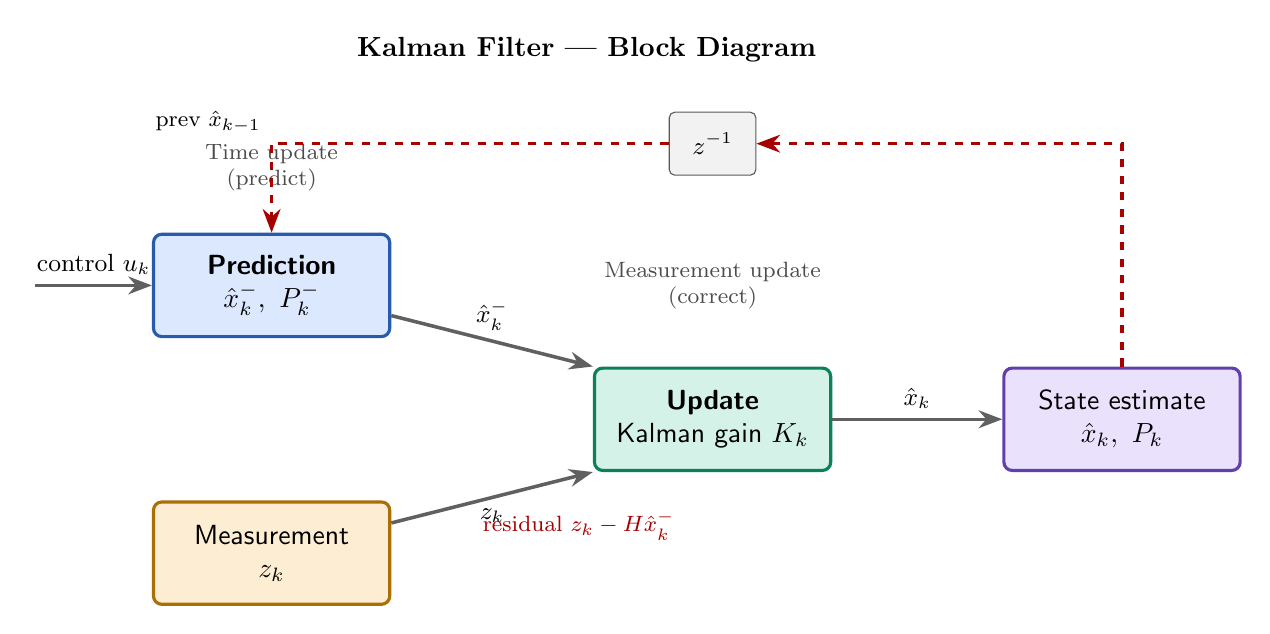
\begin{tikzpicture}[
  >={Stealth[length=3mm]},font=\sffamily,
  box/.style={rectangle,rounded corners=3pt,draw=#1!70!black,fill=#1!18,
              line width=0.4mm,minimum width=30mm,minimum height=13mm,align=center},
  sig/.style={->,line width=0.45mm,draw=gray!75!black},
  fb/.style={->,line width=0.45mm,draw=red!65!black,dashed},
]
  \definecolor{cpred}{HTML}{3B82F6}
  \definecolor{cupd}{HTML}{10B981}
  \definecolor{cmeas}{HTML}{F59E0B}
  \definecolor{cstate}{HTML}{8B5CF6}

  % nodes
  \node[box=cmeas] (meas) at (0,0) {Measurement\\$z_k$};
  \node[box=cpred] (pred) at (0,3.4) {\textbf{Prediction}\\$\hat{x}_k^- ,\ P_k^-$};
  \node[box=cupd]  (upd)  at (5.6,1.7) {\textbf{Update}\\Kalman gain $K_k$};
  \node[box=cstate](state)at (10.8,1.7){State estimate\\$\hat{x}_k ,\ P_k$};

  % time update self note
  \node[align=center,font=\footnotesize,gray!60!black] at (0,4.9)
    {Time update\\(predict)};
  \node[align=center,font=\footnotesize,gray!60!black] at (5.6,3.4)
    {Measurement update\\(correct)};

  % signal flow
  \draw[sig] (pred) -- node[above,font=\small]{$\hat{x}_k^-$} (upd.north west);
  \draw[sig] (meas) -- node[below,font=\small]{$z_k$} (upd.south west);
  \draw[sig] (upd) -- node[above,font=\small]{$\hat{x}_k$} (state);

  % residual annotation near update input
  \node[red!65!black,font=\footnotesize] at (3.9,0.35) {residual $z_k-H\hat{x}_k^-$};

  % feedback: state -> next prediction (z^{-1} delay)
  \node[draw=gray!70!black,fill=gray!10,rounded corners=2pt,font=\small,
        minimum width=11mm,minimum height=8mm] (delay) at (5.6,5.2) {$z^{-1}$};
  \draw[fb] (state.north) |- (delay.east);
  \draw[fb] (delay.west) -| node[above left,font=\footnotesize]{prev $\hat{x}_{k-1}$} (pred.north);

  % external input u_k into prediction
  \draw[sig] (-3.0,3.4) -- node[above,font=\small]{control $u_k$} (pred.west);

  \node[font=\bfseries] at (4.0,6.4) {Kalman Filter — Block Diagram};
\end{tikzpicture}
\end{document}
